\documentclass{article}
\usepackage[utf8]{inputenc}
\usepackage[a4paper, total={6in, 8in}]{geometry}
\usepackage{longtable}
\usepackage{gensymb}
\usepackage{graphicx}
\usepackage{siunitx}
\usepackage{caption}
\usepackage[colorlinks,bookmarks=false,citecolor=blue,linkcolor=blue,urlcolor=blue]{hyperref}
\usepackage{relsize}
\usepackage{amsmath}
\usepackage{amssymb}
\usepackage{bm}
\usepackage{multirow}
\usepackage{placeins}
\begin{document}
\begin{titlepage}
\begin{center}

\includegraphics[scale=0.12]{document/niser.png}
\line(1,0){340}\\
[1mm]
\begin{large}
\textbf{\huge Splitting of Sodium D-lines \\ \normalsize using diffraction grating}\\ 
\end{large}
\line(1,0){200}\\
[5cm]
\large MAITREY SHARMA\\
\small (1911093)\\
[3.5cm]
Third Year Integrated M.Sc.\\
\textbf{School of Physical Sciences}\\
\textbf{National Institute of Science Education and Research, Bhubaneshwar}\\
\small October 12, 2021
\end{center} 
\end{titlepage}
\newpage
\section{Aim}
Measurement of the wavelength separation of sodium D-lines using a diffraction grating and to calculate the angular dispersive power of the grating.

\section{Apparatus}
\begin{enumerate}
    \item Spectrometer,
    \item A prism,
    \item Diffraction grating,
    \item A sodium lamp with power supply. 
\end{enumerate}

\section{Introduction}
\noindent
The \textit{emission spectrum} of a chemical element or chemical compound is the spectrum of frequencies of electromagnetic radiation emitted due to an atom or molecule making a transition from a high energy state to a lower energy state. The photon energy of the emitted photon is equal to the energy difference between the two states. There are many possible electron transitions for each atom, and each transition has a specific energy difference. This collection of different transitions, leading to different radiated wavelengths, make up an emission spectrum. 
\par
\noindent
The observations of emission spectra began in 1756 when Thomas Melvill observed the emission of distinct patterns of colour when salts were added to alcohol flames. By 1785, James Gregory discovered the principles of diffraction grating and American astronomer David Rittenhouse made the first engineered diffraction grating. A \textbf{\textit{diffraction grating}} is an optical component with a periodic structure that splits and diffracts light into several beams travelling in different directions.
\par
\noindent
The sodium spectrum is dominated by the bright 
doublet known as the sodium D-lines at $\SI{589.0}{\nano \metre}$ and $\SI{589.6}{\nano \metre}$ as shown in figure (\ref{fig:nalines}).
\begin{figure}[h!]
    \centering
    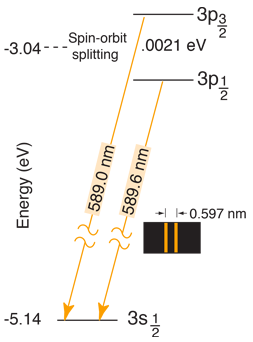
\includegraphics[scale = 0.5]{Figures/sodiumdlines.png}
    \caption{Sodium D-lines}
    \label{fig:nalines}
\end{figure}
This appears as an absorption line in many types of stars, including the Sun. The line was first studied in 1814 by Joseph von Fraunhofer during his investigation of the lines in the solar spectrum, now known as the Fraunhofer lines. Fraunhofer named it the 'D' line, although it is now known to actually be a group of closely spaced lines split by a fine and hyperfine structure.
\par
\noindent
Using an appropriate diffraction grating the wavelength separation of these two lines can be determined. A schematic for diffraction of sodium light (Na-D lines) with a plane transmission grating is shown in figure (\ref{fig:schematic}).
\begin{figure}[]
    \centering
    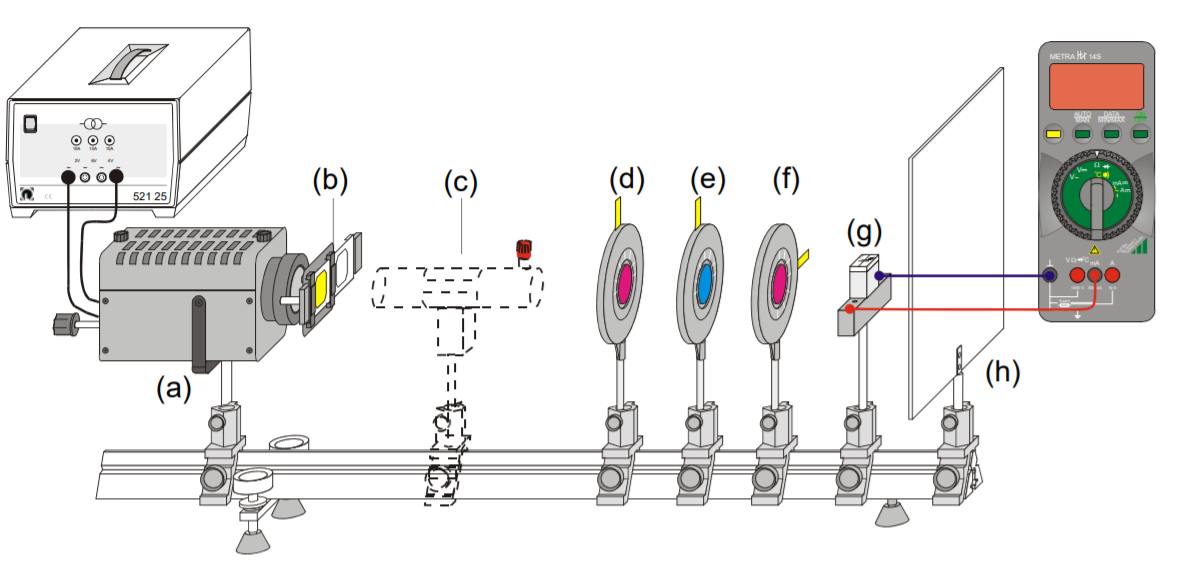
\includegraphics{Figures/schematic.png}
    \caption{Schematic for diffraction of sodium Na-D lines}
    \label{fig:schematic}
\end{figure}
\clearpage

\section{Setup}
\noindent
An arrangement consisting of a large number of parallel slits of the same width and 
separated by equal opaque spaces is known as diffraction grating. It is usually made by 
ruling equidistant, extremely close tine grooves with a diamond point on an optically
plane glass plate. A photographic replica of a plate made in this way is often used as a commercial transmission grating. The actual experimental set up is shown in figure (\ref{fig:setup}).
\begin{figure}[]
    \centering
    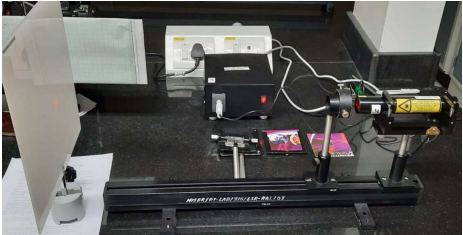
\includegraphics[scale = 0.65]{Figures/setup.png}
    \captionsetup{justification=centering}
    \caption{Experimental set up}
    \label{fig:setup}
\end{figure}



\section{Theory}
\noindent 
For $N$ parallel slits, each with a width $e$ and separated by an opaque space of width 
$b$, the diffraction pattern consists of diffraction modulated interference fringes. The quantity $(e+b)$ is called the \textit{grating element} and $N (= 1 / (e+b))$ is the number of slits per unit length, which could typically be 300 to 12000 lines per inch. For a large number of slits, the diffraction pattern consists of extremely sharp (practically narrow lines) principal maxima, together with weak secondary maxima in between the principal maxima. The various principal maxima are called \textit{orders}. 

\par
\noindent
For polychromatic incident light falling normally on a plane transmission grating the principal maxima for each spectral wavelength are given by
\begin{equation}
    \label{eq:poly}
    (e+b) \sin \theta = \pm m \lambda
\end{equation}
where $m$ is the order of principal maximum and $\theta$ is the angle of diffraction.
\par
\noindent
The \textit{angular dispersive power} of the grating is defined as the rate of change of angle of diffraction with the change in wavelength. It is obtained by differentiating equation (\ref{eq:poly}) and is given by
\begin{equation}
    \label{eq:power}
    \omega = \dfrac{d \theta}{d \lambda} = \dfrac{m}{(e+b) \cos \theta}
\end{equation}


\section{Observations and Results}
\begin{enumerate}
    \item Number of lines on grating, $N = \SI{1200}{\per \milli \metre}$.
    \item Order of the principal maximum, $m =1$.
    \item From the table, $\lambda_1 = \SI{581.414}{\nano \metre}$.
    \item From the table, $\lambda_2 = \SI{581.336}{\nano \metre}$.
    \item Thus, $\lambda_1 - \lambda_2 = \SI{0.078}{\nano \metre}$.
    \item Angular dispersive power, $\dfrac{d \theta}{d \lambda} = \dfrac{\theta_1 - \theta_2}{\lambda_1 - \lambda_2} = \SI{1.6782051e6}{\radian \per \metre}$.
\end{enumerate}
\begin{figure}[h!]
    \centering
    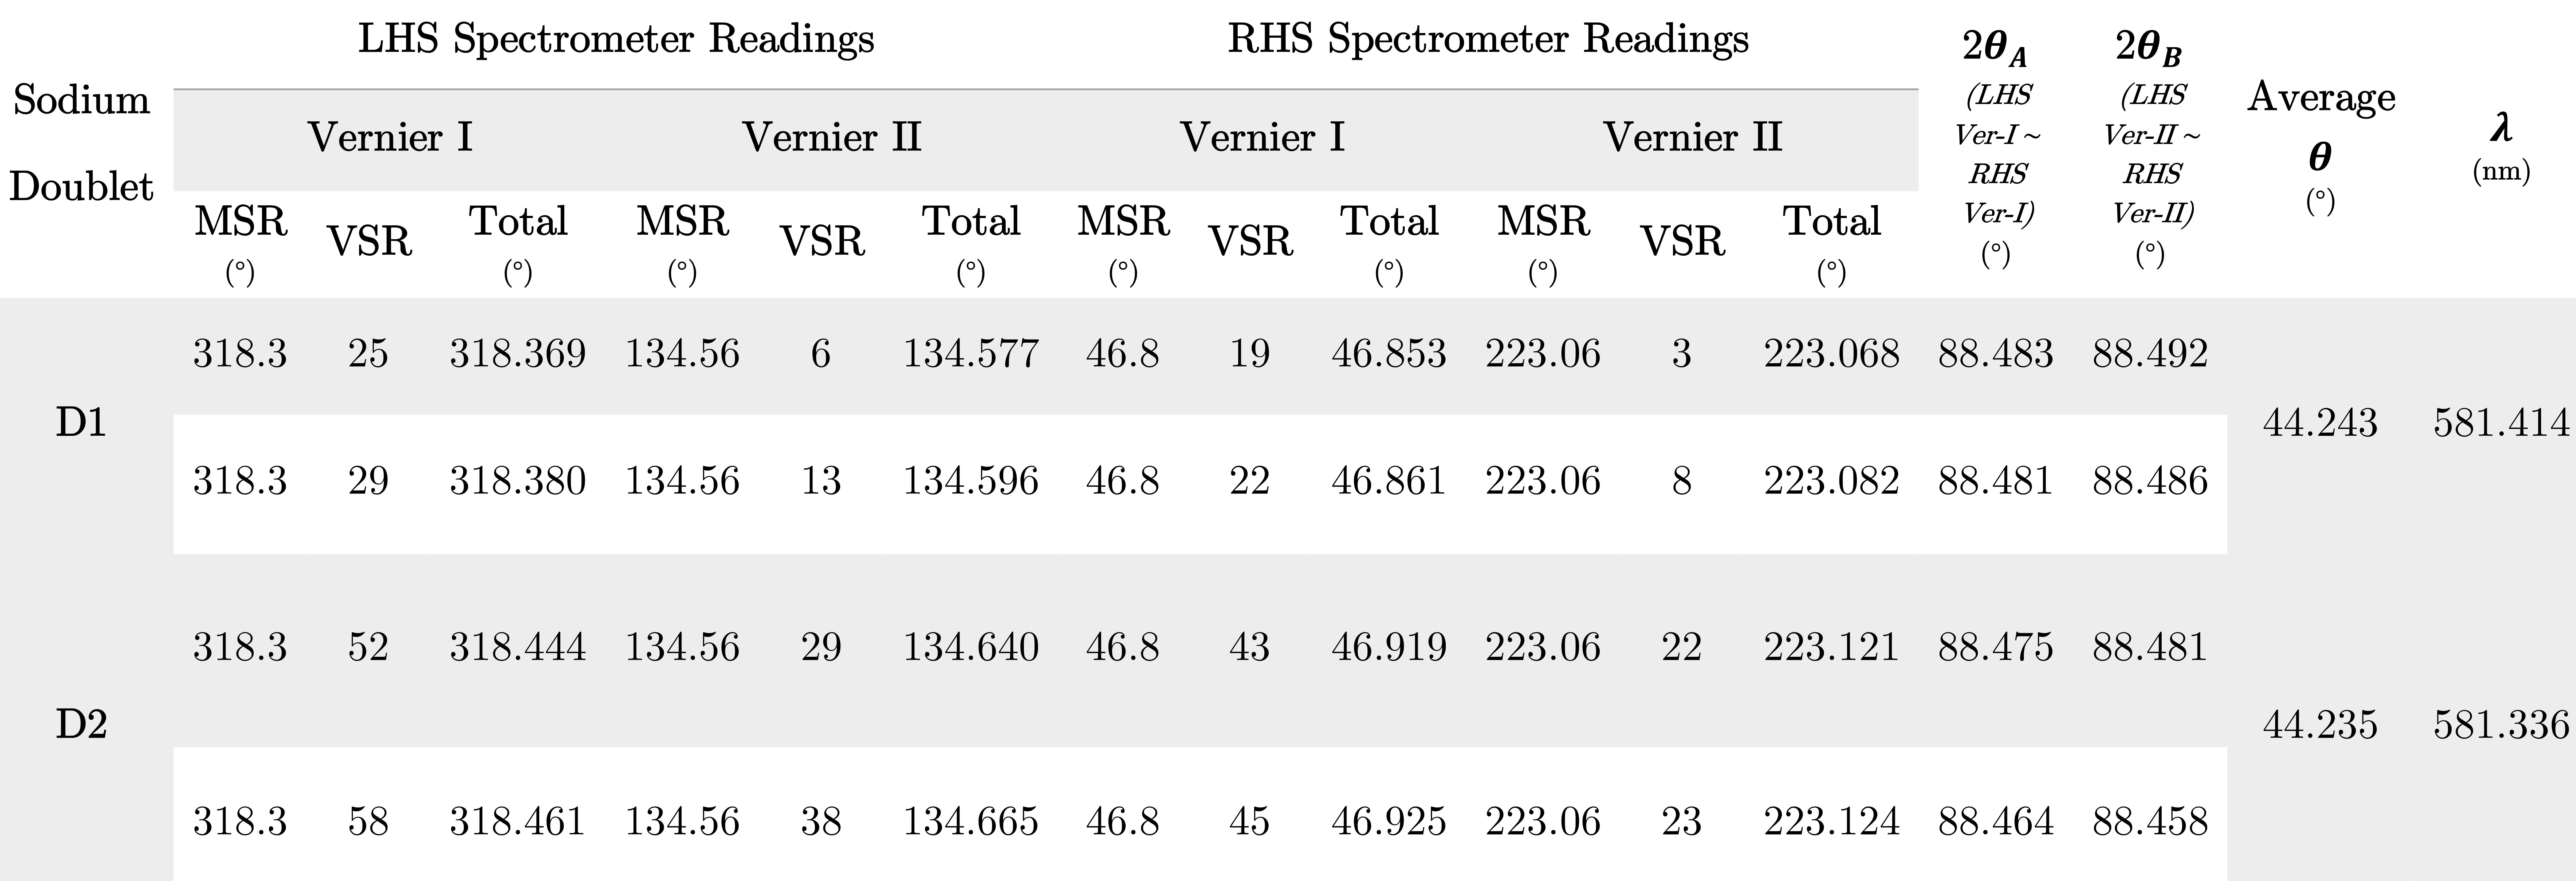
\includegraphics[scale = 0.059]{Figures/table (1).png}
    \caption{The spectrometer readings for the experiment}
    \label{tab:read}
\end{figure}


\section{Error Analysis}
The values tabulates are in degrees so we need to first convert them into radians. From here, we have
\begin{itemize}
    \item $\theta_1 = \SI{0.77217729}{\radian}$
    \item $\theta_2 = \SI{0.77204639}{\radian}$
\end{itemize}
The error analysis would be limited to the propagational errors. Now we have to find the error in $\lambda_i$'s, for that, using equation (\ref{eq:poly}), we have
\begin{equation}
    \dfrac{\delta \lambda}{\lambda} = \sqrt{\Big( \dfrac{\delta \sin \theta}{\sin \theta} \Big)^2}
\end{equation}
For this, first we need the error in $\sin \theta$, that is $\delta \sin \theta$. We know, 
\begin{equation}
    \delta \sin \theta_i = (\cos \theta_i) \cdot \delta \theta_i
\end{equation}
Now $\delta \theta$ in (degrees) is provided by the vernier constants, that is, $\Big( \dfrac{1}{360} \Big) \degree$. We convert this into radians to get
\begin{equation}
    \delta \theta = \SI{4.8481368e-5}{\radian}
\end{equation}
Therefore
\begin{equation}
    \delta \lambda_1 = 581.414 \times 10^{-9} \times \sqrt{\Big( \dfrac{\cos (0.77217729) \cdot (4.8481368 \times 10^{-5})}{\sin (0.77217729)} \Big)^2} = \SI{0.029}{\nano \metre}
\end{equation}
and
\begin{equation}
    \delta \lambda_2 = 581.336 \times 10^{-9} \times \sqrt{\Big( \dfrac{\cos (0.77204639) \cdot (4.8481368 \times 10^{-5})}{\sin (0.77204639)} \Big)^2} = \SI{0.029}{\nano \metre}
\end{equation}
And, the uncertainty in $\lambda_1 - \lambda_2$ will be consequently the summation of uncertainty in $\lambda_1$ and $\lambda_2$, that is, $\SI{0.058}{\nano \metre}$.
\par
\noindent
Now, for the error in angular dispersive power $\omega$, we have from equation (\ref{eq:power})
\begin{equation}
    \delta \omega = \omega \times \sqrt{\Big( \dfrac{\delta (\cos \theta)}{\cos \theta} \Big)^2}
\end{equation}
Note that here $\delta \cos \theta = -(\sin \theta) \cdot \delta \theta$. We will be taking average value of $\theta_1$ and $\theta_2$ for calculations. Putting in the values, we get
\begin{equation}
    \delta \omega = 1.6782051 \times 10^6 \times \sqrt{\Big( \dfrac{-0.69769980 \times 4.848136 \times 10^{-5}}{0.71643894} \Big)^2} = \SI{79.233574}{\radian \per \metre}
\end{equation}


    
    
    
\section{Results and Discussions}
\begin{enumerate}
    \item Using diffraction grating, the value of the first sodium $D$-line was found to be \\ $\lambda_1 = \SI[separate-uncertainty=true]{581.41 \pm 0.03}{\nano \metre}$ after taking care of significant figures.
    \item Using diffraction grating, the value of the second sodium $D$-line was found to be \\ $\lambda_2 = \SI[separate-uncertainty=true]{581.34 \pm 0.03}{\nano \metre}$ after taking care of significant figures.
    \item The difference in wavelengths of the sodium $D$-lines was found to be \\ $\Delta \lambda = \lambda_1 - \lambda_2 = \SI[separate-uncertainty=true]{78 \pm 58}{\pico \metre}$, which is close to that of the literature value of \SI{6}{\pico \metre} after taking care of significant figures.
    \item The angular dispersive power was found to be $\omega = \SI[separate-uncertainty=true]{1678200 \pm 80}{\radian \per \metre}$ after taking care of significant figures.
    \item One of the source of this error/ambiguity could be the way readings have been noted.
    \item Another source of error for the obtained results could be the way observations have been made since we can not definitely say when a fringe has vanished.

\end{enumerate}

\section{Precautions}
\begin{enumerate}
    \item Once the collimator and the telescope are adjusted for parallel rays, their focusing should not be disturbed throughout the experiment. 
    \item Once the grating is properly adjusted on the turntable it should be locked. 
    \item While taking measurements at different positions of the telescope. It must always be in locked condition. 
    \item While rotating the telescope arm if the vernier crosses over $0 \degree$ ($360 \degree$) on the circular main scale take the angular difference appropriately.
\end{enumerate}
\end{document}
